\documentclass{article}
\usepackage[utf8]{inputenc}
\usepackage[dvipsnames]{xcolor}
\usepackage{amsmath, amsthm, amssymb, amscd, amsxtra,color,authblk,tikz,arydshln,array, caption, romannum,verbatim,enumitem}
\usetikzlibrary{shapes,arrows,positioning}
\usepackage[T1]{fontenc}
\usetikzlibrary{decorations.markings}

\begin{document}

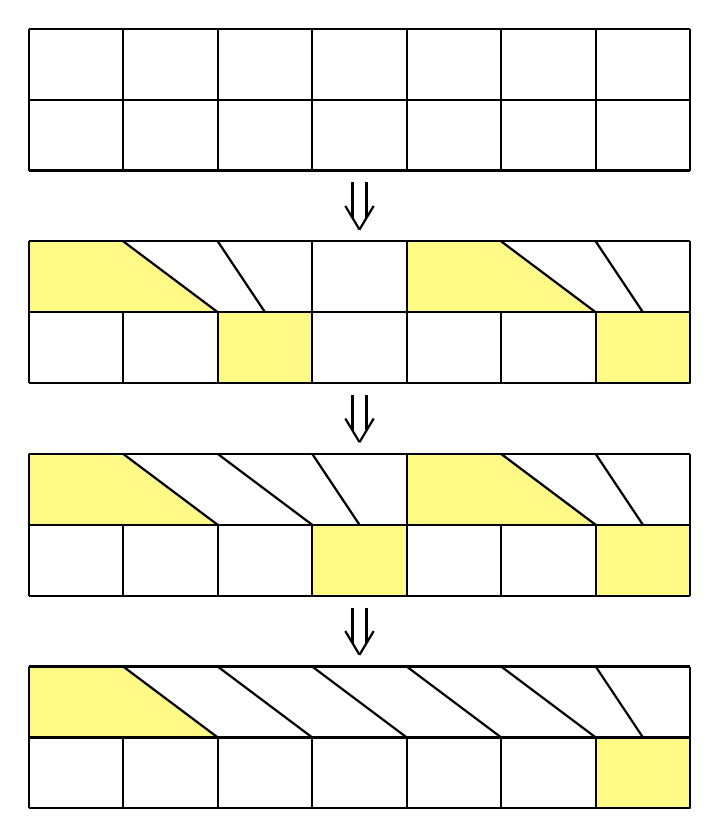
\begin{tikzpicture}[scale=0.3]
\foreach \j in {-10.5, -1.5, 7.5}
        \draw[black, fill=yellow!80, opacity=0.6] (0,{\j}) -- (4,{\j}) -- (8,{\j-3}) -- (0,{\j-3}) -- cycle;
\foreach \j in {-1.5, 7.5}
        \draw[black, fill=yellow!80, opacity=0.6] (16,{\j}) -- (20,{\j}) -- (24,{\j-3}) -- (16,{\j-3}) -- cycle;
\foreach \j in {-13.5, -4.5, 4.5}
        \draw[black, fill=yellow!80, opacity=0.6] (24,{\j}) -- (28,{\j}) -- (28,{\j-3}) -- (24,{\j-3}) -- cycle;
\draw[black, fill=yellow!80, opacity=0.6] (8,4.5) -- (12,4.5) -- (12,1.5) -- (8,1.5) -- cycle;
\draw[black, fill=yellow!80, opacity=0.6] (12,-4.5) -- (16,-4.5) -- (16,-7.5) -- (12,-7.5) -- cycle;

\foreach \j in {-16.5,-13.5,-10.5,-7.5,-4.5,-1.5,1.5,4.5,7.5,10.5,13.5,16.5}
        \draw[thick, black] (0,{\j}) -- (28,{\j});        
\foreach \i in {0, 4, 8, 12, 16, 20, 24, 28}
\foreach \j in {-16.5, -7.5, 1.5, 10.5, 13.5}
        \draw[thick, black] ({\i},{\j}) -- ({\i},{\j+3});

\foreach \j in {-13.5, -4.5, 4.5}
        \draw[thick, black] (0,{\j}) -- (0,{\j+3});
\foreach \j in {-13.5, -4.5, 4.5}
        \draw[thick, black] (28,{\j}) -- (28,{\j+3});
\foreach \j in {-13.5, -4.5, 4.5}
        \draw[thick, black] (26,{\j}) -- (24,{\j+3});
\foreach \j in {-4.5, 4.5}
        \draw[thick, black] (24,{\j}) -- (20,{\j+3});
\foreach \j in {-4.5, 4.5}
        \draw[thick, black] (16,{\j}) -- (16,{\j+3});
\foreach \j in {-4.5, 4.5}
        \draw[thick, black] (8,{\j}) -- (4,{\j+3});
\foreach \i in {4, 8, 12, 16, 20}
        \draw[thick, black] ({\i},-10.5) -- ({\i+4},-13.5);
\draw[thick, black] (12,4.5) -- (12,7.5);
\draw[thick, black] (10,4.5) -- (8,7.5);
\draw[thick, black] (14,-4.5) -- (12,-1.5);
\draw[thick, black] (12,-4.5) -- (8,-1.5);

\foreach \i in {13.7, 14.3}
\foreach \j in {-8, 1, 10}
        \draw[thick, black] ({\i},{\j}) -- ({\i},{\j-1.5});
\foreach \j in {-10, -1, 8}
        \draw[thick, black] (14,{\j}) -- (14.6,{\j+1});
\foreach \j in {-10, -1, 8}
        \draw[thick, black] (14,{\j}) -- (13.4,{\j+1});
\end{tikzpicture}

\end{document}